\subsection{绘制垫片特征图}
\begin{procedure}
\item 设置图层。

新建“中心线”和“实线”两个图层,具体设计请参看\ref{sec:dianpian}节的图层设置相关内容。
\item  切换视图为主视图。
\item 绘制中心线。

中心线绘制结果如图\ref{fig:dianpiancenterline1}所示。
绘制对称中心线。
\begin{lstlisting}
|命令: xline|
|指定点或 [水平(H)/垂直(V)/角度(A)/二等分(B)/偏移(O)]:|
|指定通过点:$@1<0$|
|指定通过点:$@1<90$|
|指定通过:|
\end{lstlisting}
通过偏移的方法产生$\phi 8$圆孔的中心线。
\begin{lstlisting}
|命令:OFFSET|
|当前设置: 删除源=否  图层=源  OFFSETGAPTYPE=0|
|指定偏移距离或 [通过(T)/删除(E)/图层(L)] $<$通过$>$:  42|
|选择要偏移的对象,或 [退出(E)/放弃(U)] $<$退出$>$:|
|指定要偏移的那一侧上的点,或 [退出(E)/多个(M)/放弃(U)] $<$退出$>$:|
|选择要偏移的对象,或 [退出(E)/放弃(U)] $<$退出$>$:
\end{lstlisting}
\item 将图层切换为实线层
\begin{figure}[htbp]
\centering
\subfloat[]{\label{fig:dianpiancenterline1}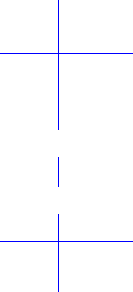
\includegraphics[scale=0.6]{dianpiancenterline1.png}}\hspace{40pt}
\subfloat[]{\label{fig:dianpianleft1}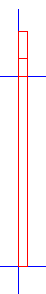
\includegraphics[scale=0.6]{dianpianleft1.png}}
\caption{垫片特征图绘制}
\end{figure}
\item 绘用于旋转操作的关键特征。

使用【矩形】命令绘制左视图中的关键特征,其结果如图\ref{fig:dianpianleft1}所示。绘制用于旋转产生$\phi 104$直径圆柱的特征矩形。
\begin{lstlisting}
|命令: rectang|
|指定第一个角点或 [倒角(C)/标高(E)/圆角(F)/厚度(T)/宽度(W)]:|
|指定另一个角点或 [面积(A)/尺寸(D)/旋转(R)]: @2,52|
\end{lstlisting}
绘制用于旋转生成$\phi 8$直径圆柱的特征矩形。
\begin{lstlisting}
|命令: rectang|
|指定第一个角点或 [倒角(C)/标高(E)/圆角(F)/厚度(T)/宽度(W)]:|
|指定另一个角点或 [面积(A)/尺寸(D)/旋转(R)]: @2,4|
\end{lstlisting}
绘制用于旋转生成$\phi 53$直径圆柱的特征矩形。
\begin{lstlisting}
|命令: rectang|
|指定第一个角点或 [倒角(C)/标高(E)/圆角(F)/厚度(T)/宽度(W)]:|
|指定另一个角点或 [面积(A)/尺寸(D)/旋转(R)]: @2,26.5|
\end{lstlisting}
\end{procedure}

\endinput